\begin{equation}
    \vec{B} - \vec{A} = \myvec{1\\4\\-4}, \vec{C} - \vec{A} = \myvec{2\\8\\-8}
\end{equation}
Forming the matrix $\vec{M}$,
\begin{align}
    \vec{M}=\myvec{\vec{B} - \vec{A} & \vec{C} - \vec{A}}^\top
\end{align}
\begin{align}
=\myvec{1 &4 &-4\\2 &8 &-8}
\end{align}
Using matrix transformation,
\begin{align}
 \vec{M} = \begin{pmatrix}
    1 & 4 & -4\\
    2 & 8 & -8
    \end{pmatrix} \xleftrightarrow{\text{$R_2$}\rightarrow{\text{$R_2 - {2} R_1$ }}}
 \begin{pmatrix}
 1 & 4 & -4\\
 0 & 0 & 0
 \end{pmatrix}
\end{align}
 
\begin{equation}
   \implies rank(\vec{M}) = 1 
\end{equation}
Thus $\vec{A}$, $\vec{B}$ and $\vec{C}$ are collinear as can be seen in Fig. \ref{aug/2/12/plot}.

 
\begin{figure}[!ht]
    \centering 
         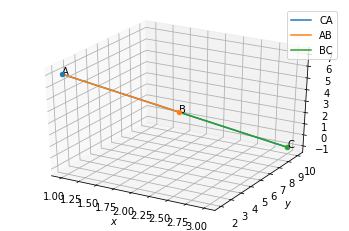
\includegraphics[width=\columnwidth]{solutions/aug/2/12/Figure.png}
         \caption{Plot}
         \label{aug/2/12/plot}
\end{figure}
